\startappendix{\madgraph Generated Feynman Diagrams}
\label{app:madgraph_diagrams}
For any processes that are sampled using \madgraph, the resulting diagrams used are all displayed here.

\section{Muon Decay}
\label{app:muon_diagrams}
These are all the Feynman diagrams when doing the muon decay calculation.
Here we sample the background, the scalar signal, and also the dark photon signal.

\subsection{Standard Model Background}
All background diagrams sampled are shown in Fig.\ \ref{fig:mu_eeenunu_bkg}. 
Note that some of these diagrams have multiple $W$ propagators, and will be heavily suppressed by an extra factor of $G_F^2$ compared to the diagrams with a single $W$.
There are also diagrams which were omitted carrying a $Z$ instead of a photon, and of course the Higgs diagrams are excluded without any loss of accuracy.

\begin{figure}[p]
    \centering
    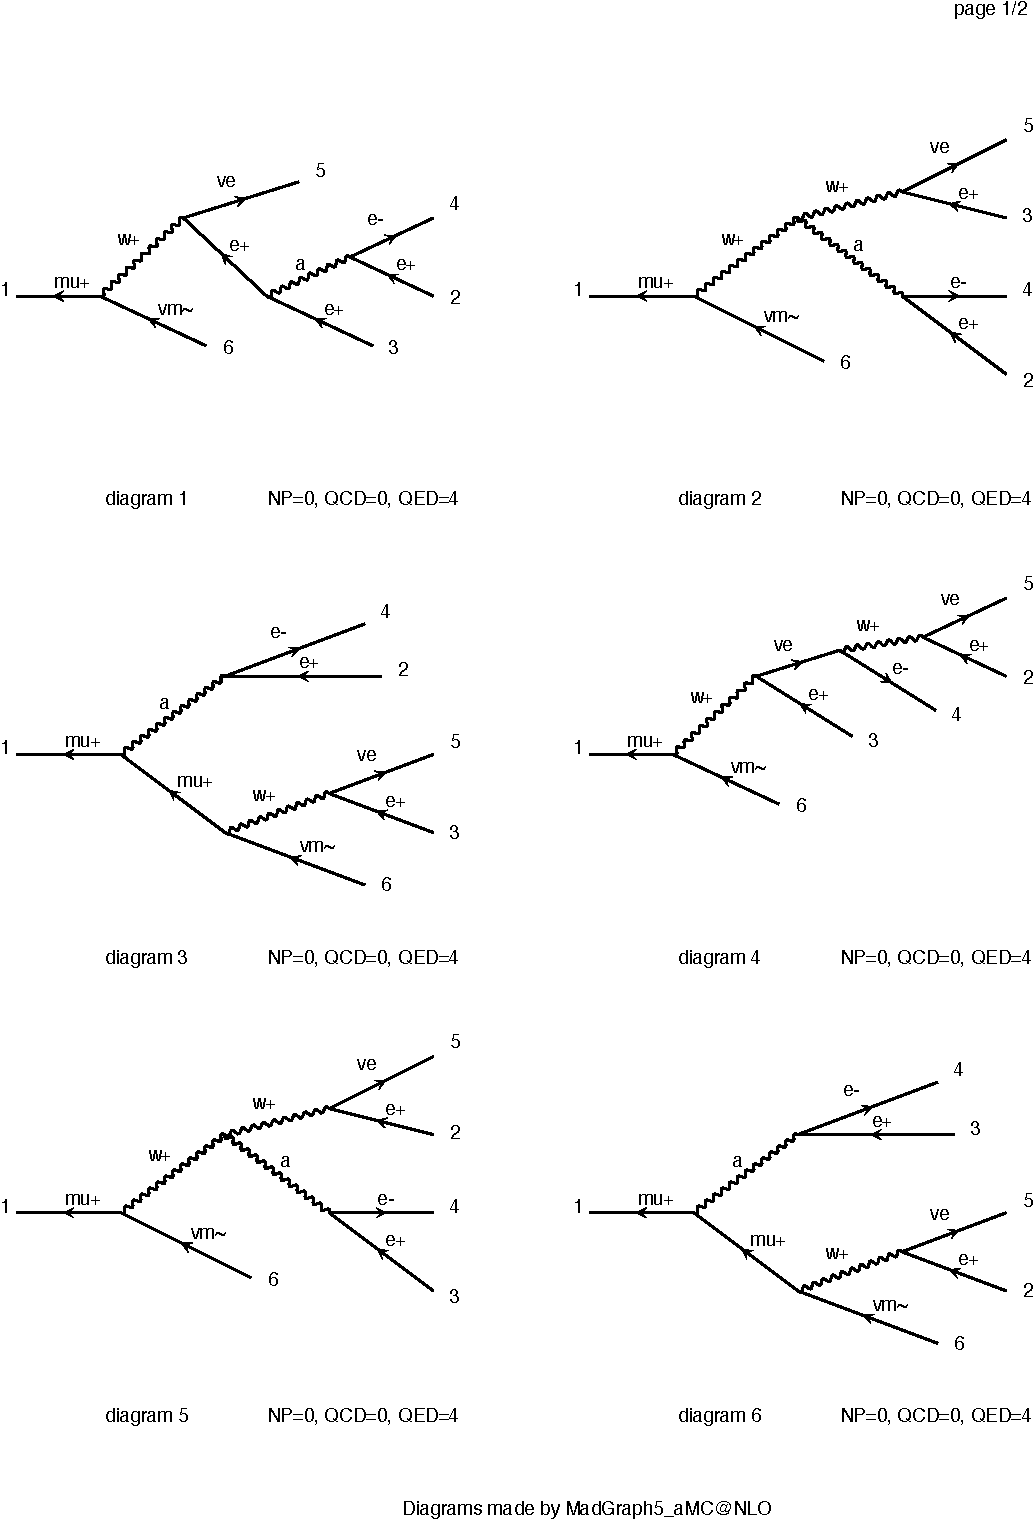
\includegraphics[width=\textwidth,clip=true,viewport=0 540 500 680,page=1]{Figures/madgraph_diagrams/mu_eeenunu_background.pdf}
    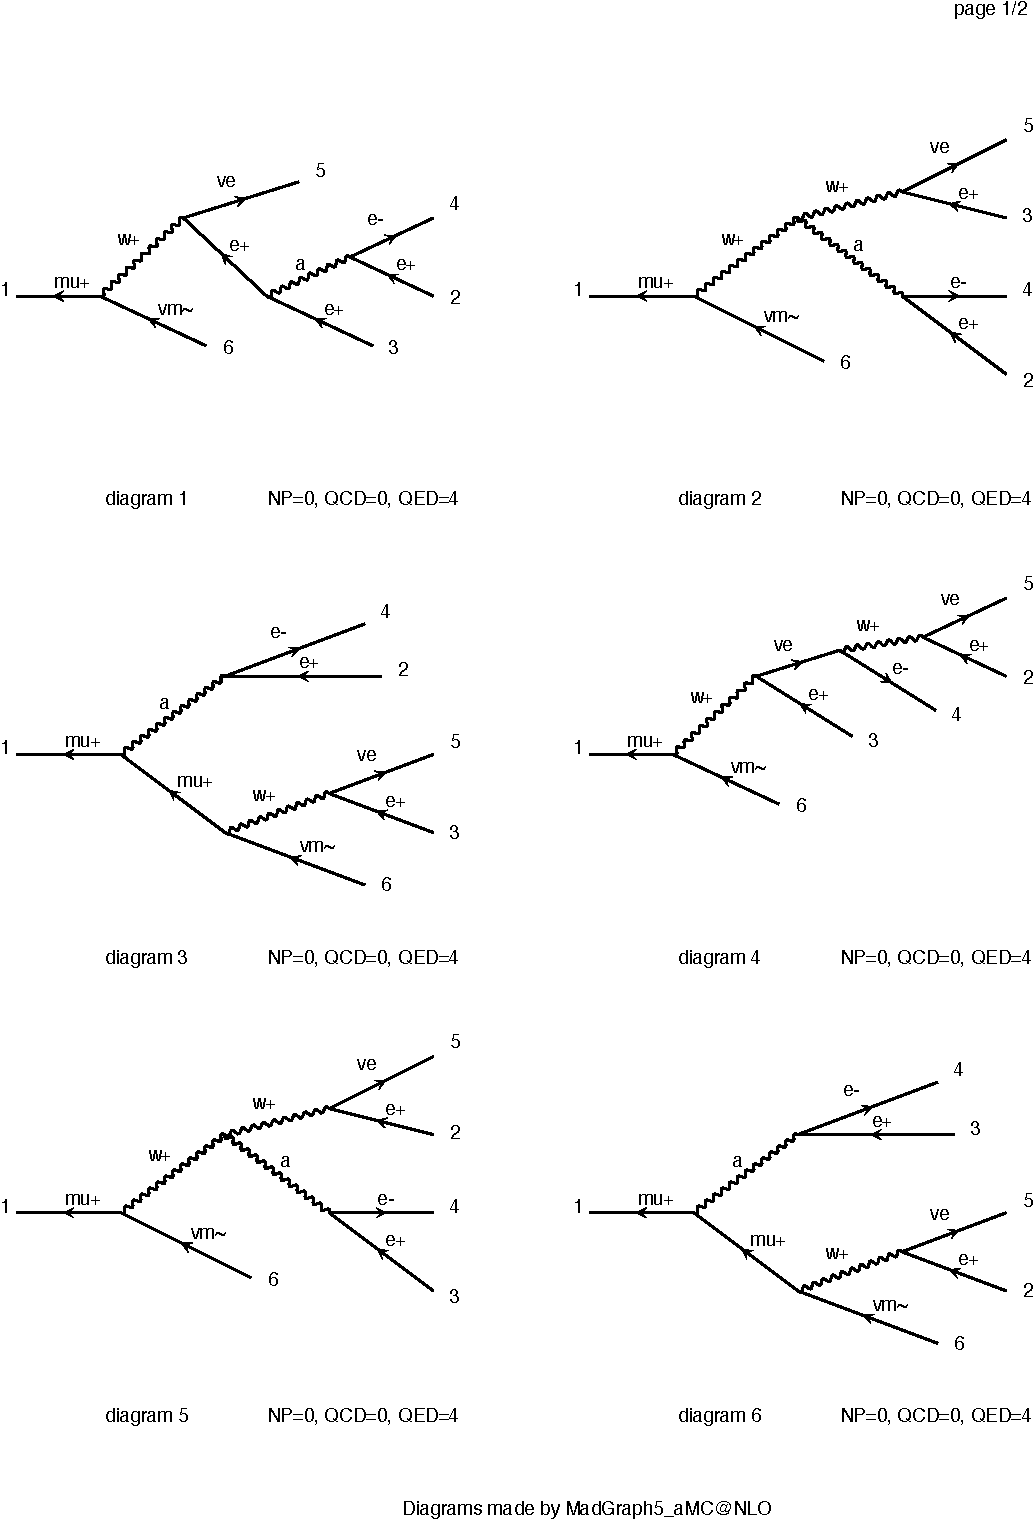
\includegraphics[width=\textwidth,clip=true,viewport=0 300 500 460,page=1]{Figures/madgraph_diagrams/mu_eeenunu_background.pdf}
    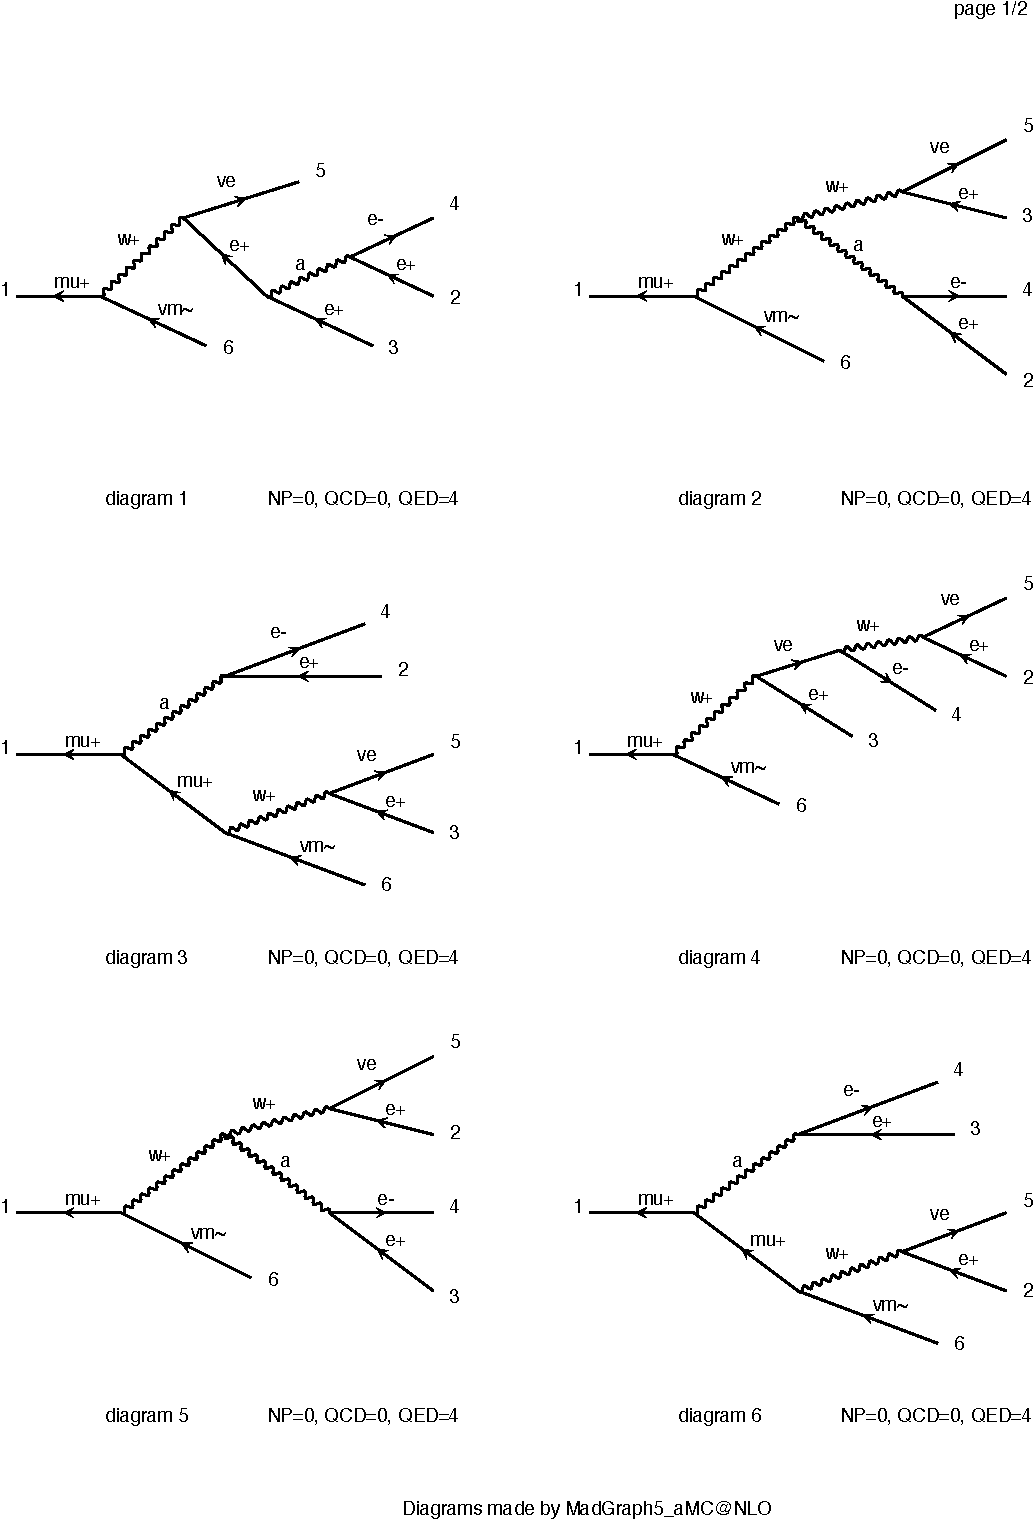
\includegraphics[width=\textwidth,clip=true,viewport=0  70 500 250,page=1]{Figures/madgraph_diagrams/mu_eeenunu_background.pdf}
    \includegraphics[width=\textwidth,clip=true,viewport=0 550 500 690,page=2]{Figures/madgraph_diagrams/mu_eeenunu_background.pdf}
    \caption{SM background contribution to muon decay with an extra $e^+ e^-$ pair in the final state. Nothing is required to be on-shell here by default.}
    \label{fig:mu_eeenunu_bkg}
\end{figure}

\subsection{Scalar Signal}
All signal diagrams sampled for the scalar are shown in Fig.\ \ref{fig:mu_eee_scalar}.
In these diagrams, keep in mind that the scalar is required to be \emph{on-shell}.
It is also assumed that the scalar has a narrow width and will decay promptly.
This restricts the number of diagrams and also forces \madgraph to compute the decay as a decay chain instead of a single decay.

\begin{figure}[h]
    \centering
    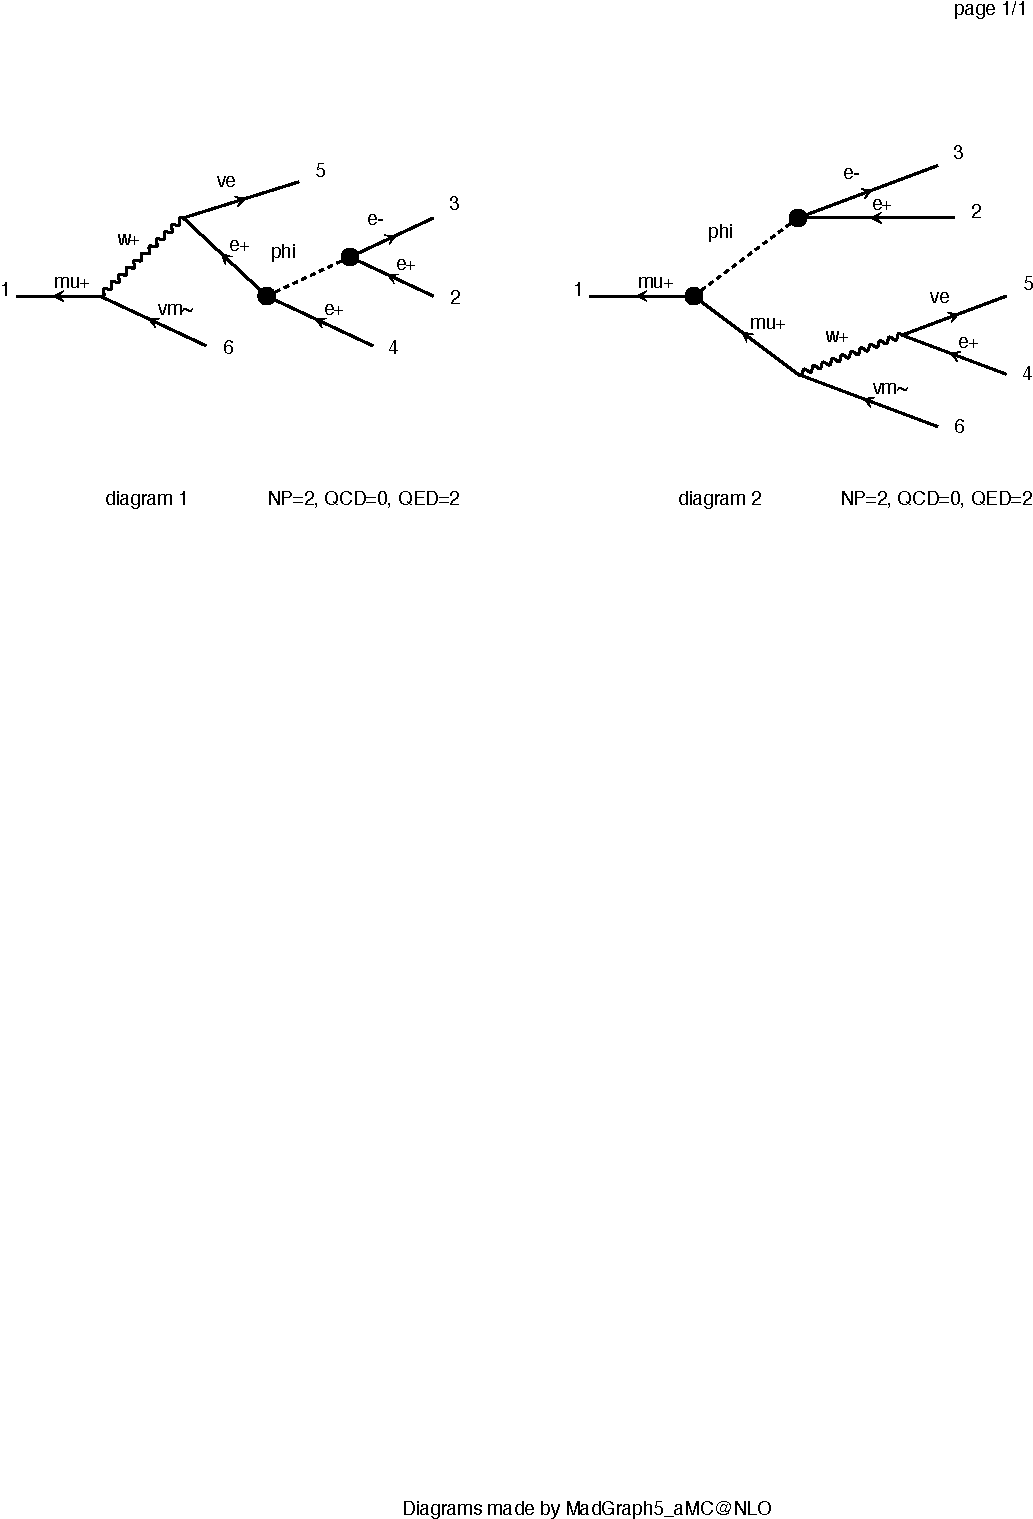
\includegraphics[width=\textwidth,clip=true,viewport=0 500 500 700]{Figures/madgraph_diagrams/mu_eeenunu_scalar.pdf}
    \caption{Signal contribution to muon decay from the scalar field. The scalar is taken to be on-shell where it decays to an $e^+ e^-$ pair.}
    \label{fig:mu_eee_scalar}
\end{figure}

\subsection{Dark Photon Signal}
All signal diagrams sampled for the dark photon are shown in Fig.\ \ref{fig:mu_eee_darkphoton}.
Again, the dark photon here is required to be produced \emph{on-shell}.
The same comment regarding the width of the dark photon can be said here.

\begin{figure}[h]
    \centering
    \includegraphics[width=\textwidth,clip=true,viewport=0 500 500 700]{Figures/madgraph_diagrams/mu_eeenunu_darkphoton.pdf}
    \caption{Signal contribution to muon decay from the dark photon. The dark photon is taken to be on-shell where it decays to an $e^+ e^-$ pair.}
    \label{fig:mu_eee_darkphoton}
\end{figure}

\section{$e^+ e^-$ Collisions at B-factories}
\label{app:ee_diagrams}
Here we present all the diagrams generated by \madgraph in the calculations of $e^+ e^-$ collision cross sections.

\subsection{Standard Model Background}
We only show a portion of the diagrams in Fig.\ \ref{fig:ee_tautauee_background} for the SM background process $e^+ e^- \rightarrow \tau^+ \tau^- e^+ e^-$, as there are many diagrams.

\begin{figure}[h]
    \centering
    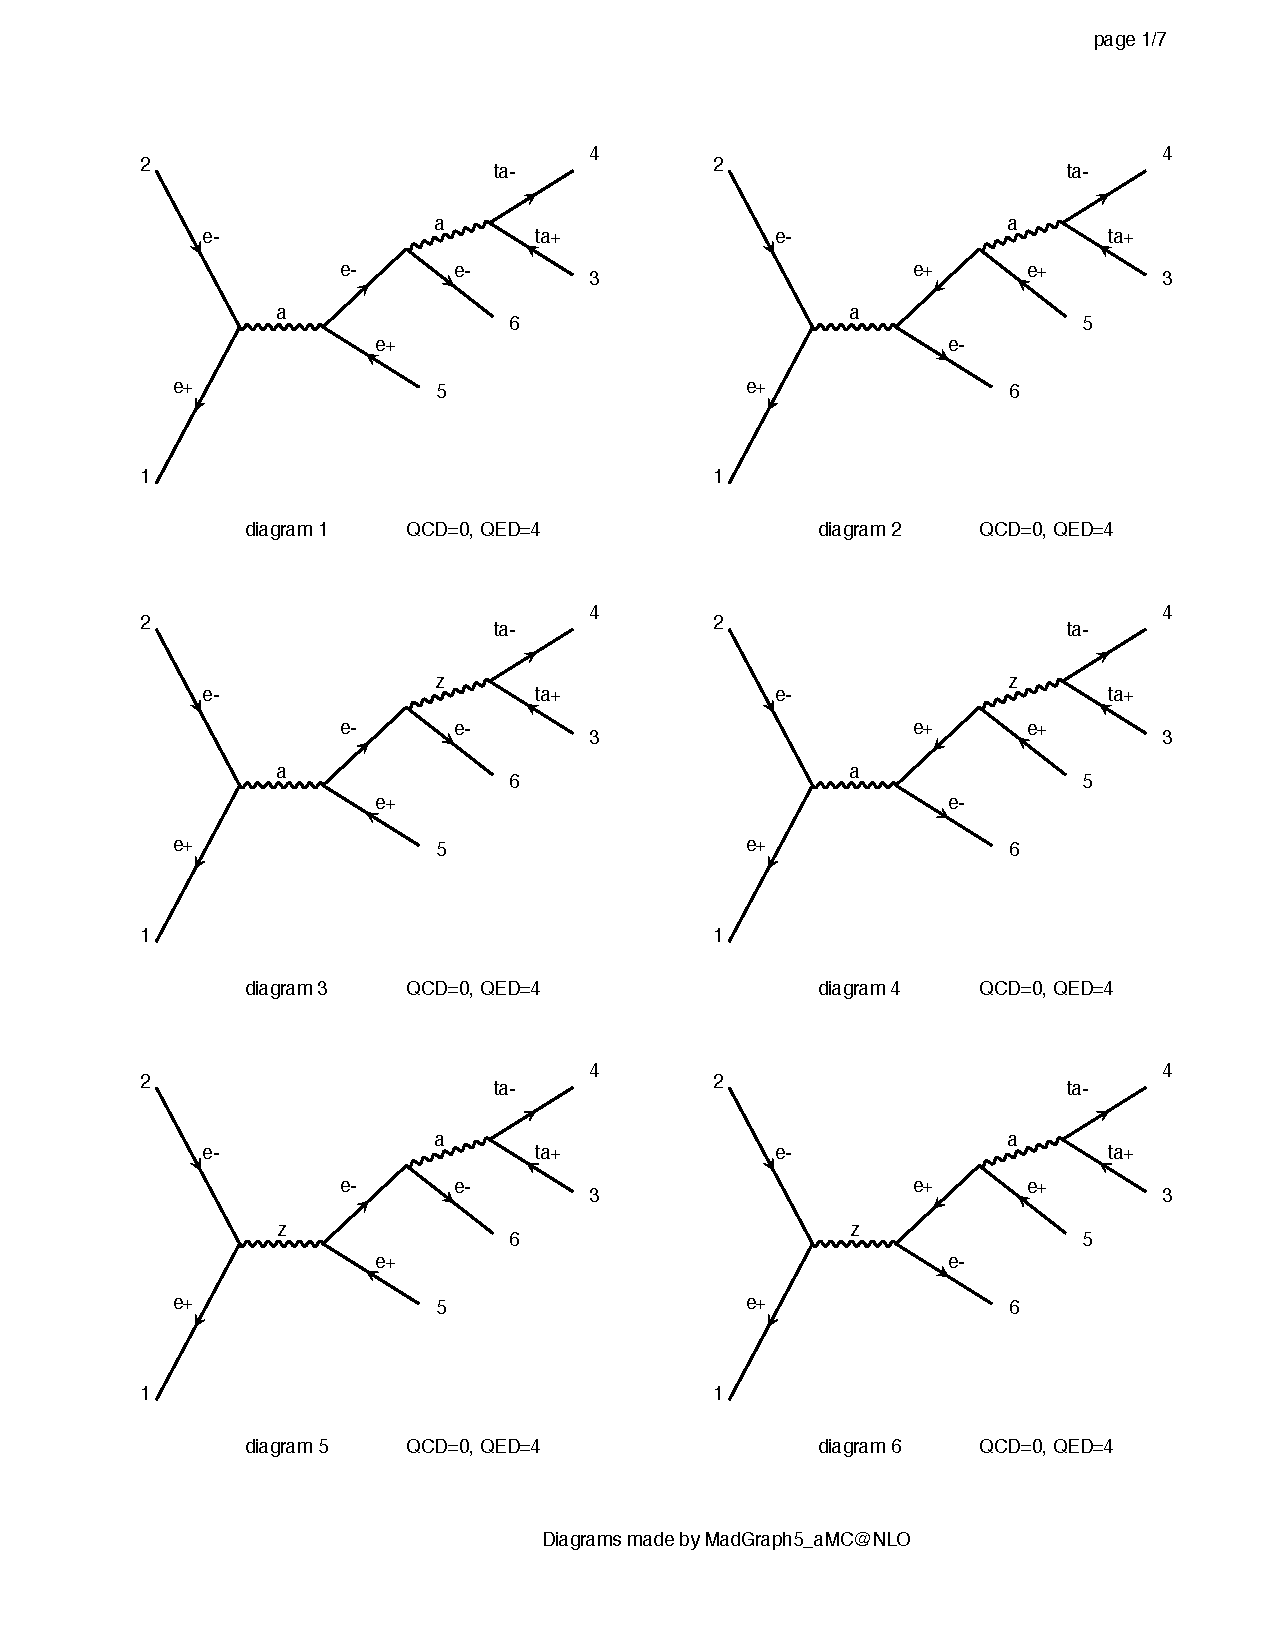
\includegraphics[width=0.45\textwidth,clip=true,viewport=65 550 315 730,page=1]{Figures/madgraph_diagrams/ee_tautauee_background.pdf}
    \includegraphics[width=0.45\textwidth,clip=true,viewport=65 110 315 310,page=3]{Figures/madgraph_diagrams/ee_tautauee_background.pdf}
    \includegraphics[width=0.45\textwidth,clip=true,viewport=65 550 315 730,page=5]{Figures/madgraph_diagrams/ee_tautauee_background.pdf}
    \includegraphics[width=0.45\textwidth,clip=true,viewport=400 220 600 340,page=6]{Figures/madgraph_diagrams/ee_tautauee_background.pdf}
    \caption{A sample collection of the diagrams generated by \madgraph for the process $e^+ e^- \rightarrow \tau^+ \tau^- e^+ e^-$. There are twists of these diagrams, replacements of the photon with a Z-boson, loops travelling in opposite directions, and also a final state with muons instead of electrons.}
    \label{fig:ee_tautauee_background}
\end{figure}

\subsection{Scalar Signal}
The diagrams shown in Fig.\ \ref{fig:ee_tautauee_scalar} are used to compute the signal portion of the study.

\begin{figure}[h]
    \centering
    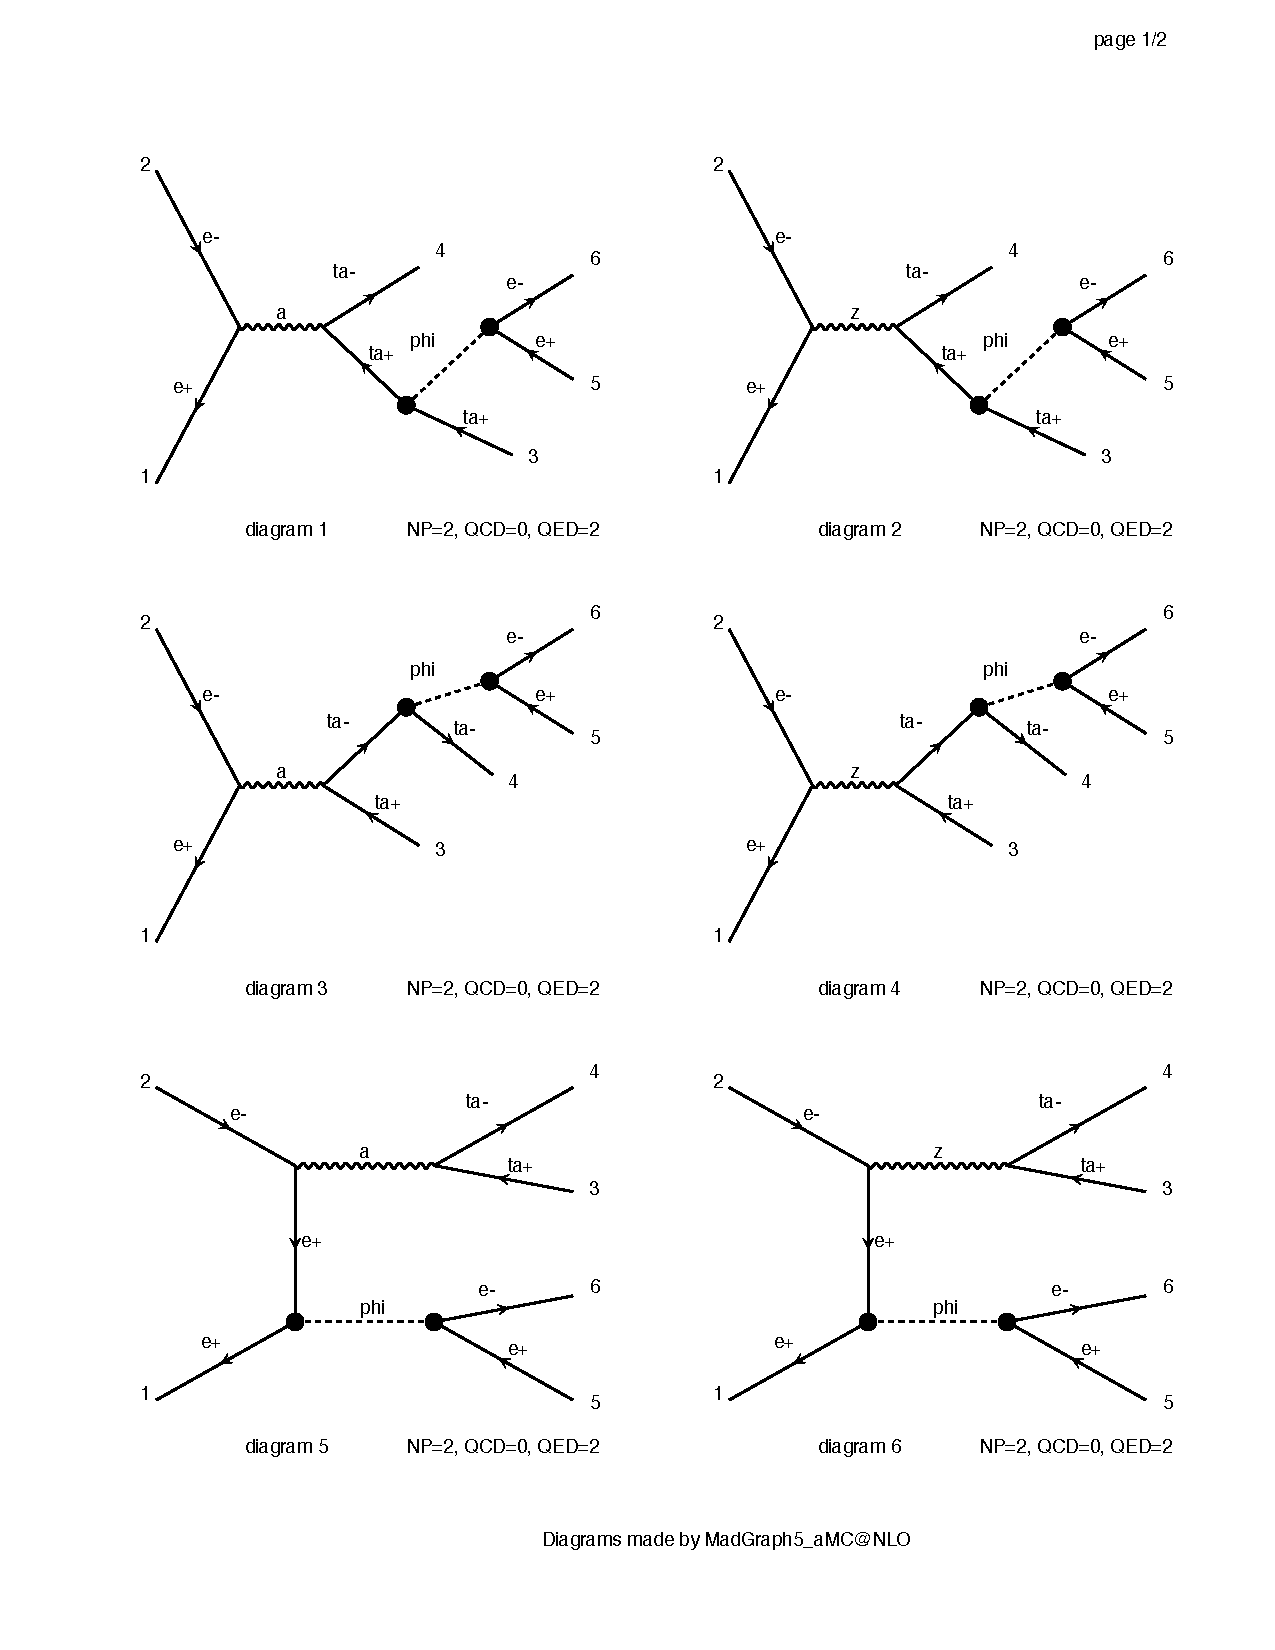
\includegraphics[width=0.45\textwidth,clip=true,viewport=65 550 315 730,page=1]{Figures/madgraph_diagrams/ee_tautauee_scalar.pdf}
    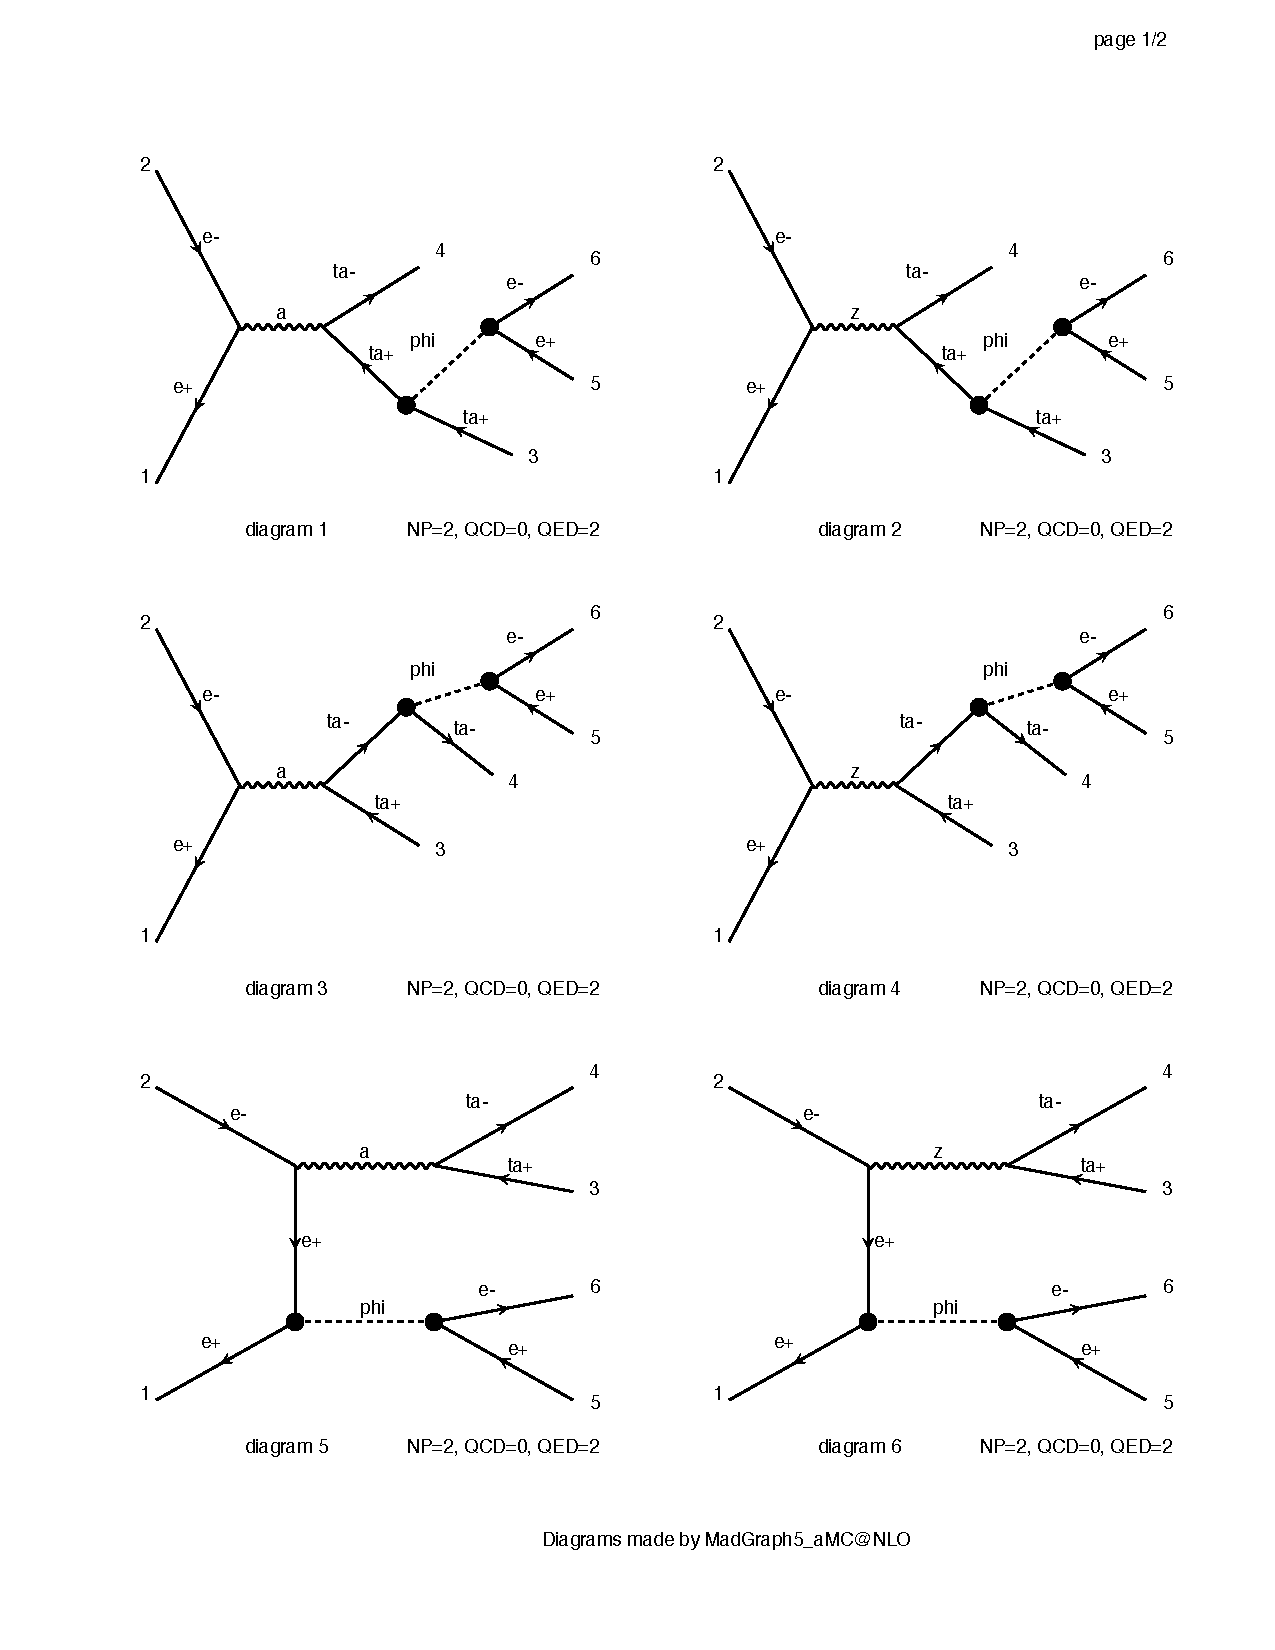
\includegraphics[width=0.45\textwidth,clip=true,viewport=65 340 315 520,page=1]{Figures/madgraph_diagrams/ee_tautauee_scalar.pdf}
    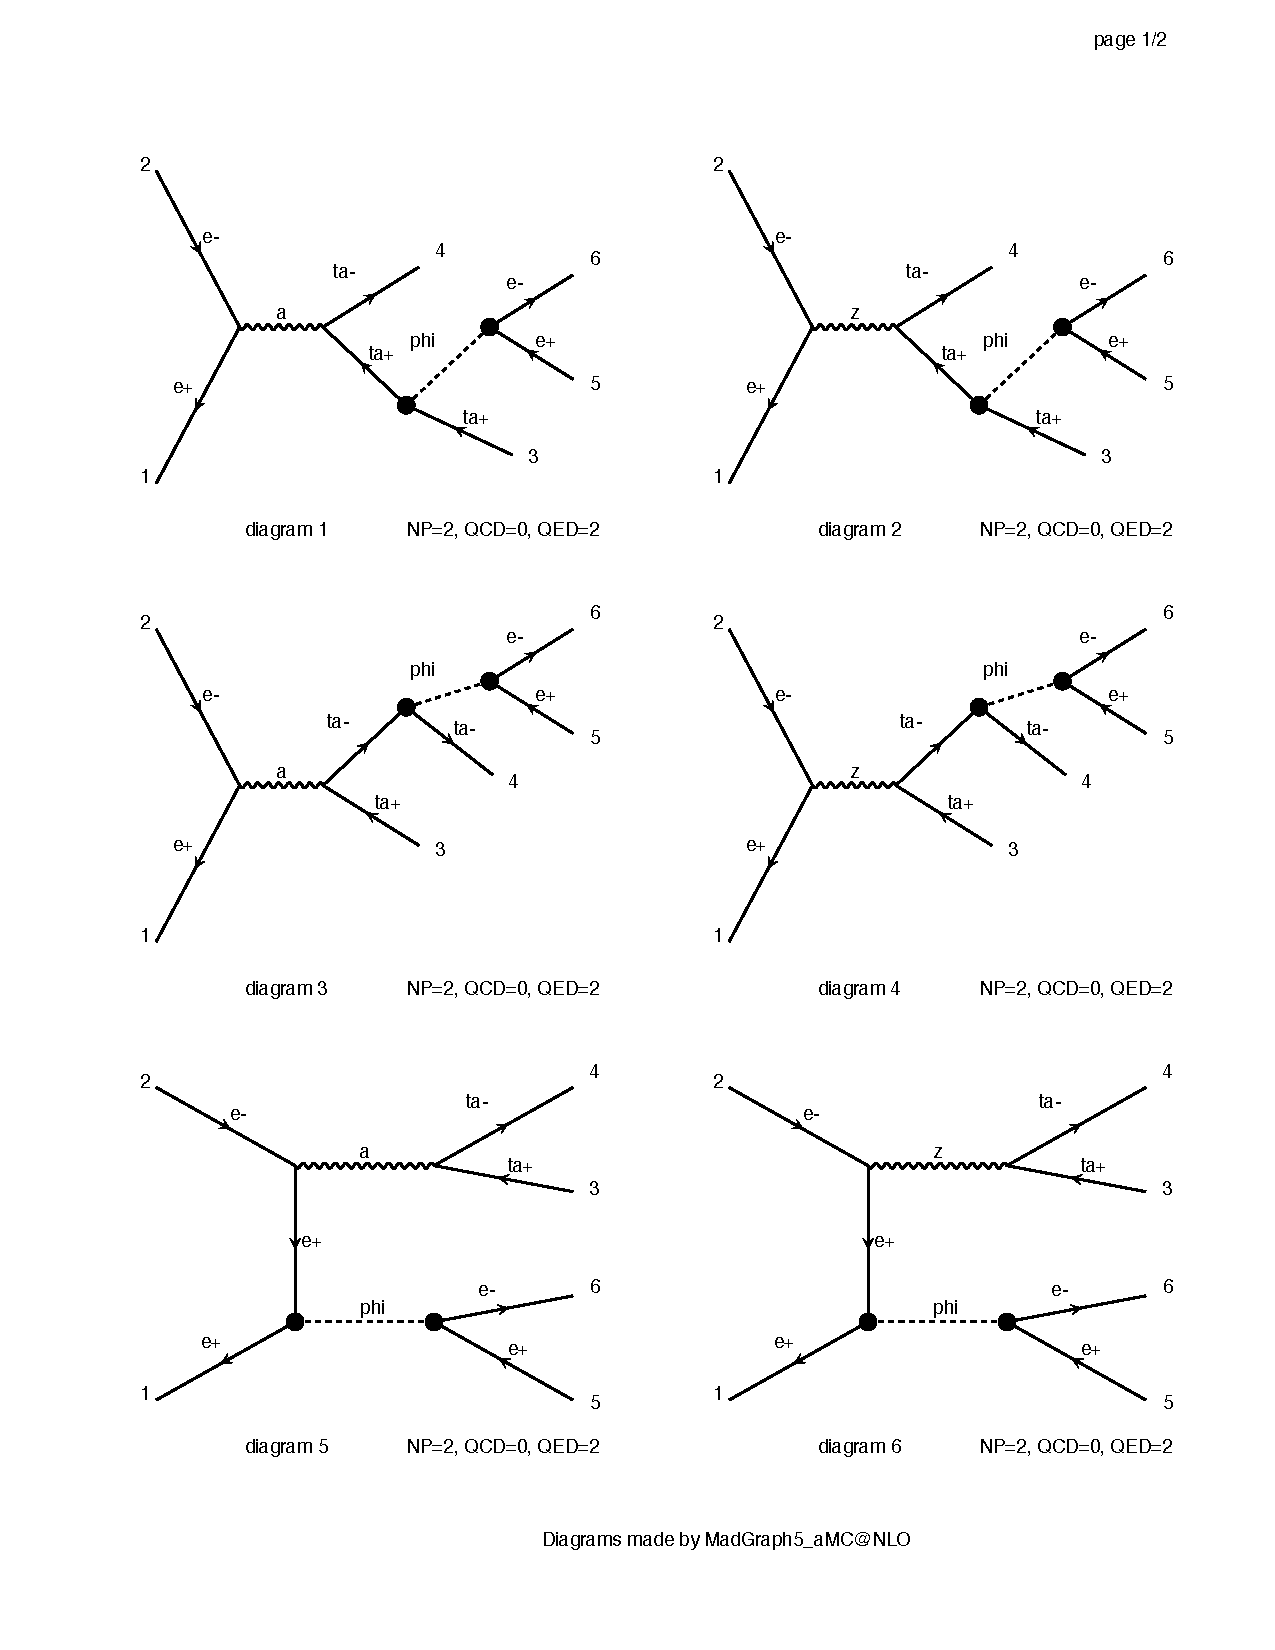
\includegraphics[width=0.45\textwidth,clip=true,viewport=65 110 315 310,page=1]{Figures/madgraph_diagrams/ee_tautauee_scalar.pdf}
    \includegraphics[width=0.45\textwidth,clip=true,viewport=65 550 315 730,page=2]{Figures/madgraph_diagrams/ee_tautauee_scalar.pdf}
    \caption{$e^+ e^-$ annihilation to $\tau^+ \tau^- e^+ e^-$. We also generate the same diagrams but with a pair $\mu^+ \mu^-$ instead in the final state. One can also replace a photon in each of the diagrams with a $Z$ to reconstruct the full set of diagrams used. The scalar is taken to be on-shell where it decays to an $e^+ e^-$ pair.}
    \label{fig:ee_tautauee_scalar}
\end{figure}
